\documentclass[12pt]{article}
\usepackage{url}
\usepackage[margin=0.5in]{geometry}
\usepackage{graphicx}
\graphicspath{ {/}}


\title{Fairbook: USSA}

\author{A. Snow, C. McKenzie, C. Yang, J. Lyons, M. Zhang}

\begin{document}
	\maketitle


	\tableofcontents
	\section{ONIDs}
		snowan, mckencod, yangco, lyonsja, zhangm4



	\section{User Stories}
	\begin{enumerate}
	\item As a User I can search for textbooks by using different search criteria so that relevant results are returned. 

	\item As a User I can add textbooks to the cart so that I can keep track of the books I am interested in.

	\item As a User I can remove textbooks I no longer want from the cart.

	\item As a User I can log in so that I can access additional features (cart, ordering). 

	\item As a User I can edit my personal account information so that it is kept up to date. 

	\item As a User I can edit my payment information so that is is kept up to date. 

	\item As a User I can filter my searches (via author, title, keyword) so that the display of unwanted materials is minimal.

	\item As a User I can select a specific book so that I can view detailed information on it.

	\item As a User I can choose which seller I want to purchase a book from, so I can get the price and condition I want. 

	\item As a Seller I can list a book for sale including condition, price, access code status, and a picture so that the information is accurate.

	\item As a Seller I can manage my current listings and remove ones I no longer want.

	\item As a Manager I can delete/ban user accounts and edit user permissions.
	\end{enumerate}



	\section{Corresponding Tasks}



	\section{UML Sequence Diagrams/Spikes}
		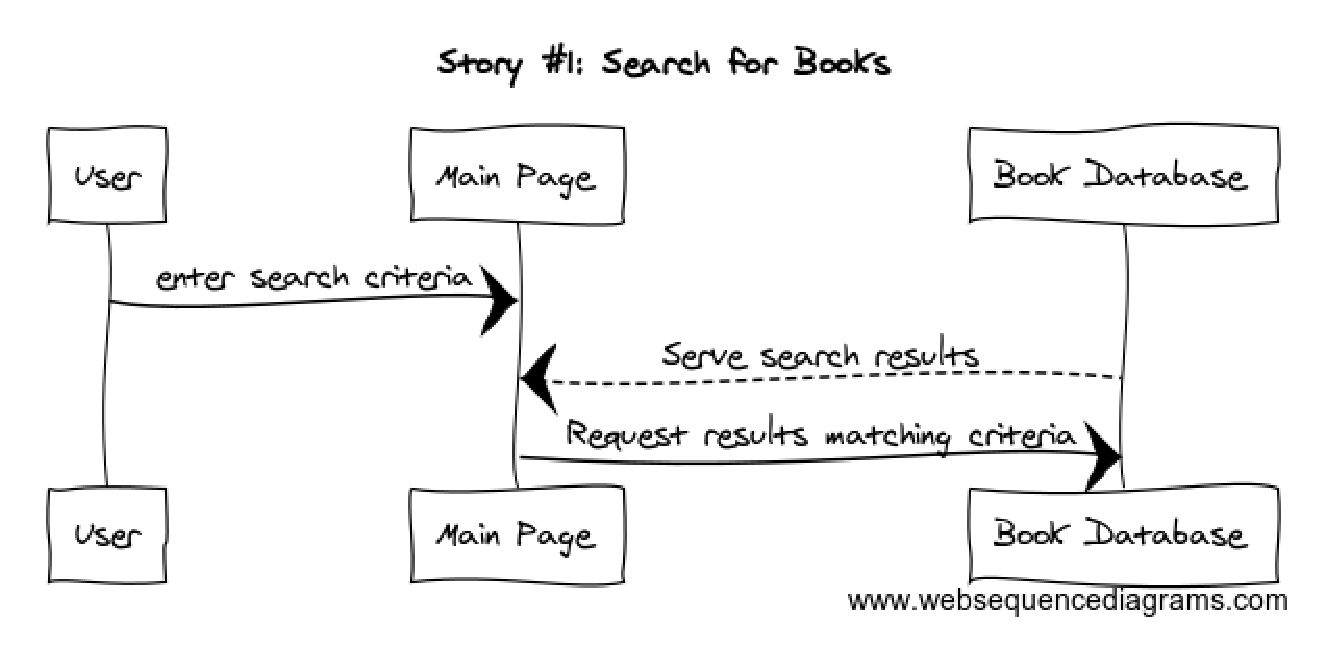
\includegraphics[width=16cm]{story1.eps}
		\par
		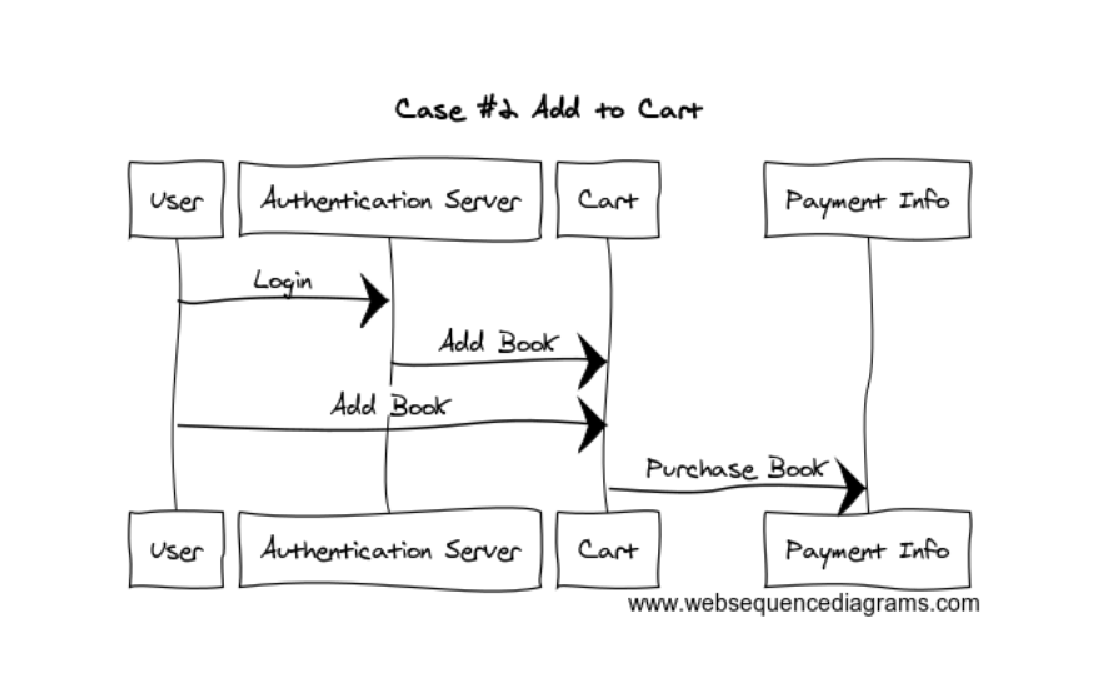
\includegraphics[width=14cm]{story2.eps}
		\par
		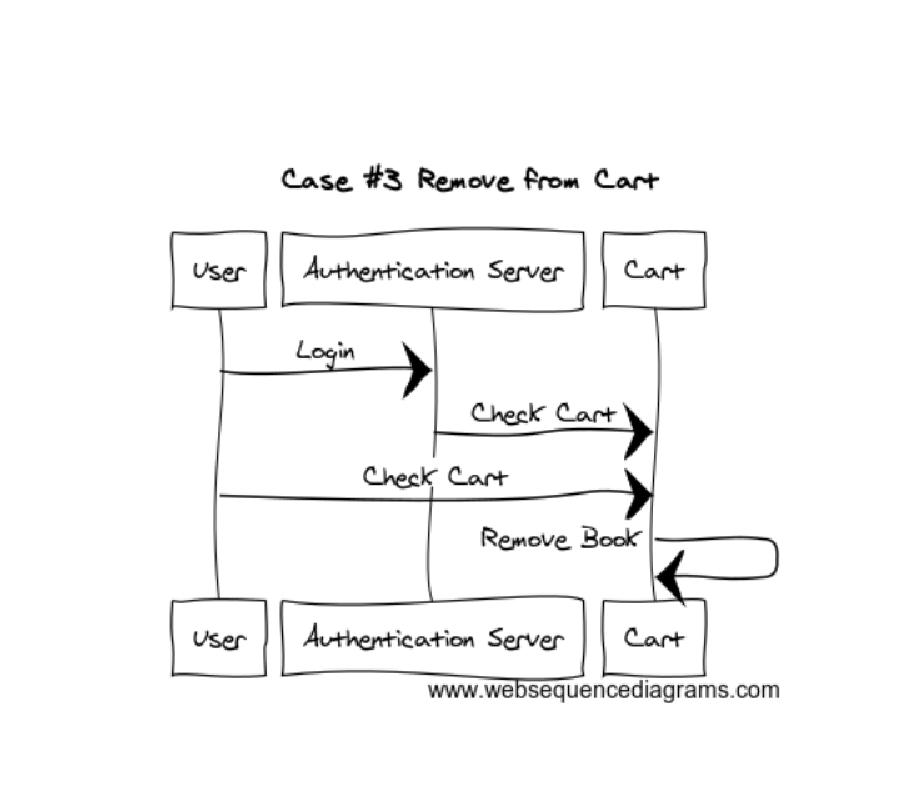
\includegraphics[width=12cm]{story3.eps}
		%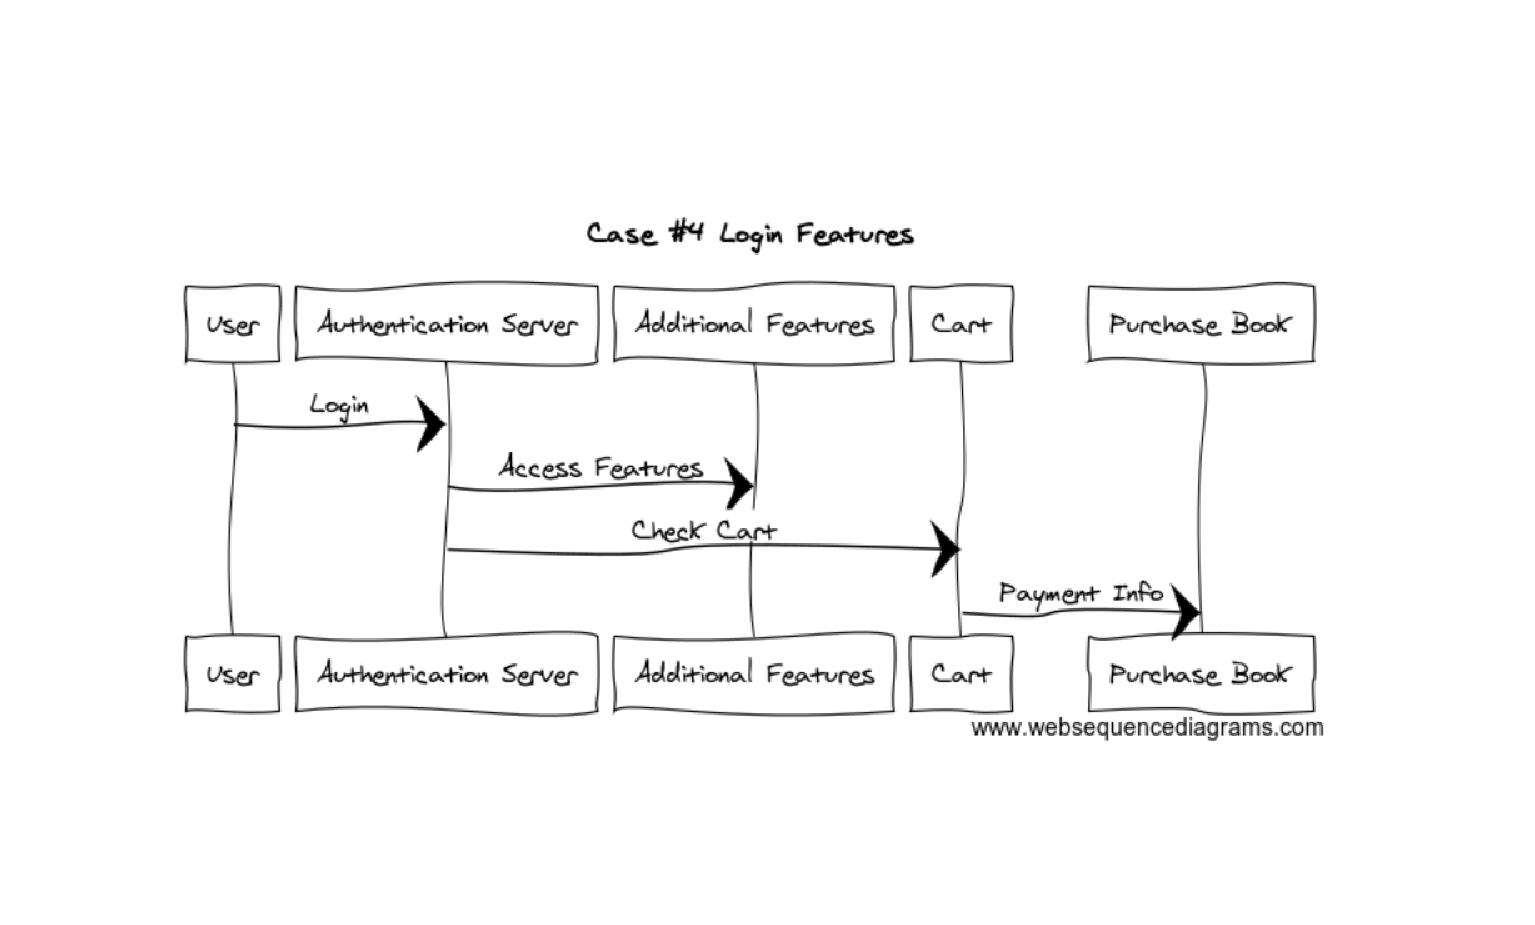
\includegraphics[width=16cm]{story4.eps}
		\par
		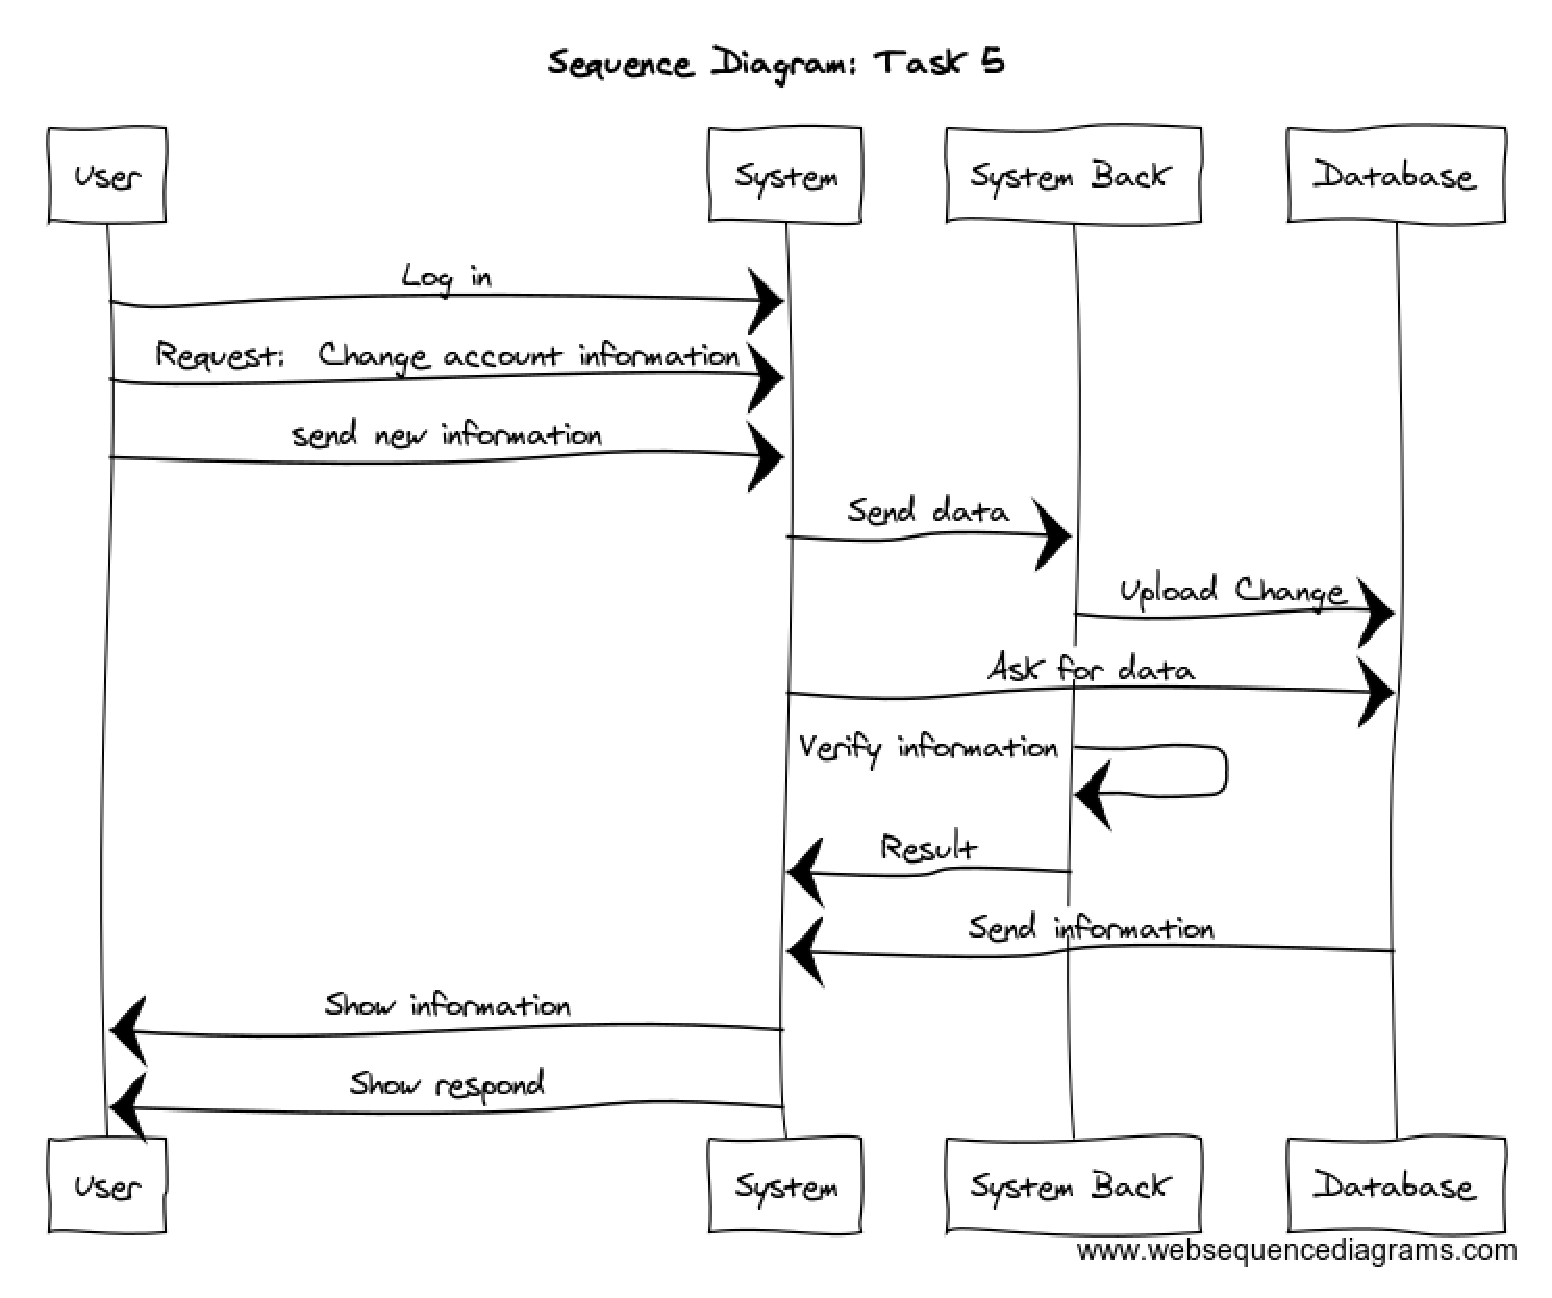
\includegraphics[width=16cm]{story5.eps}
		\par
		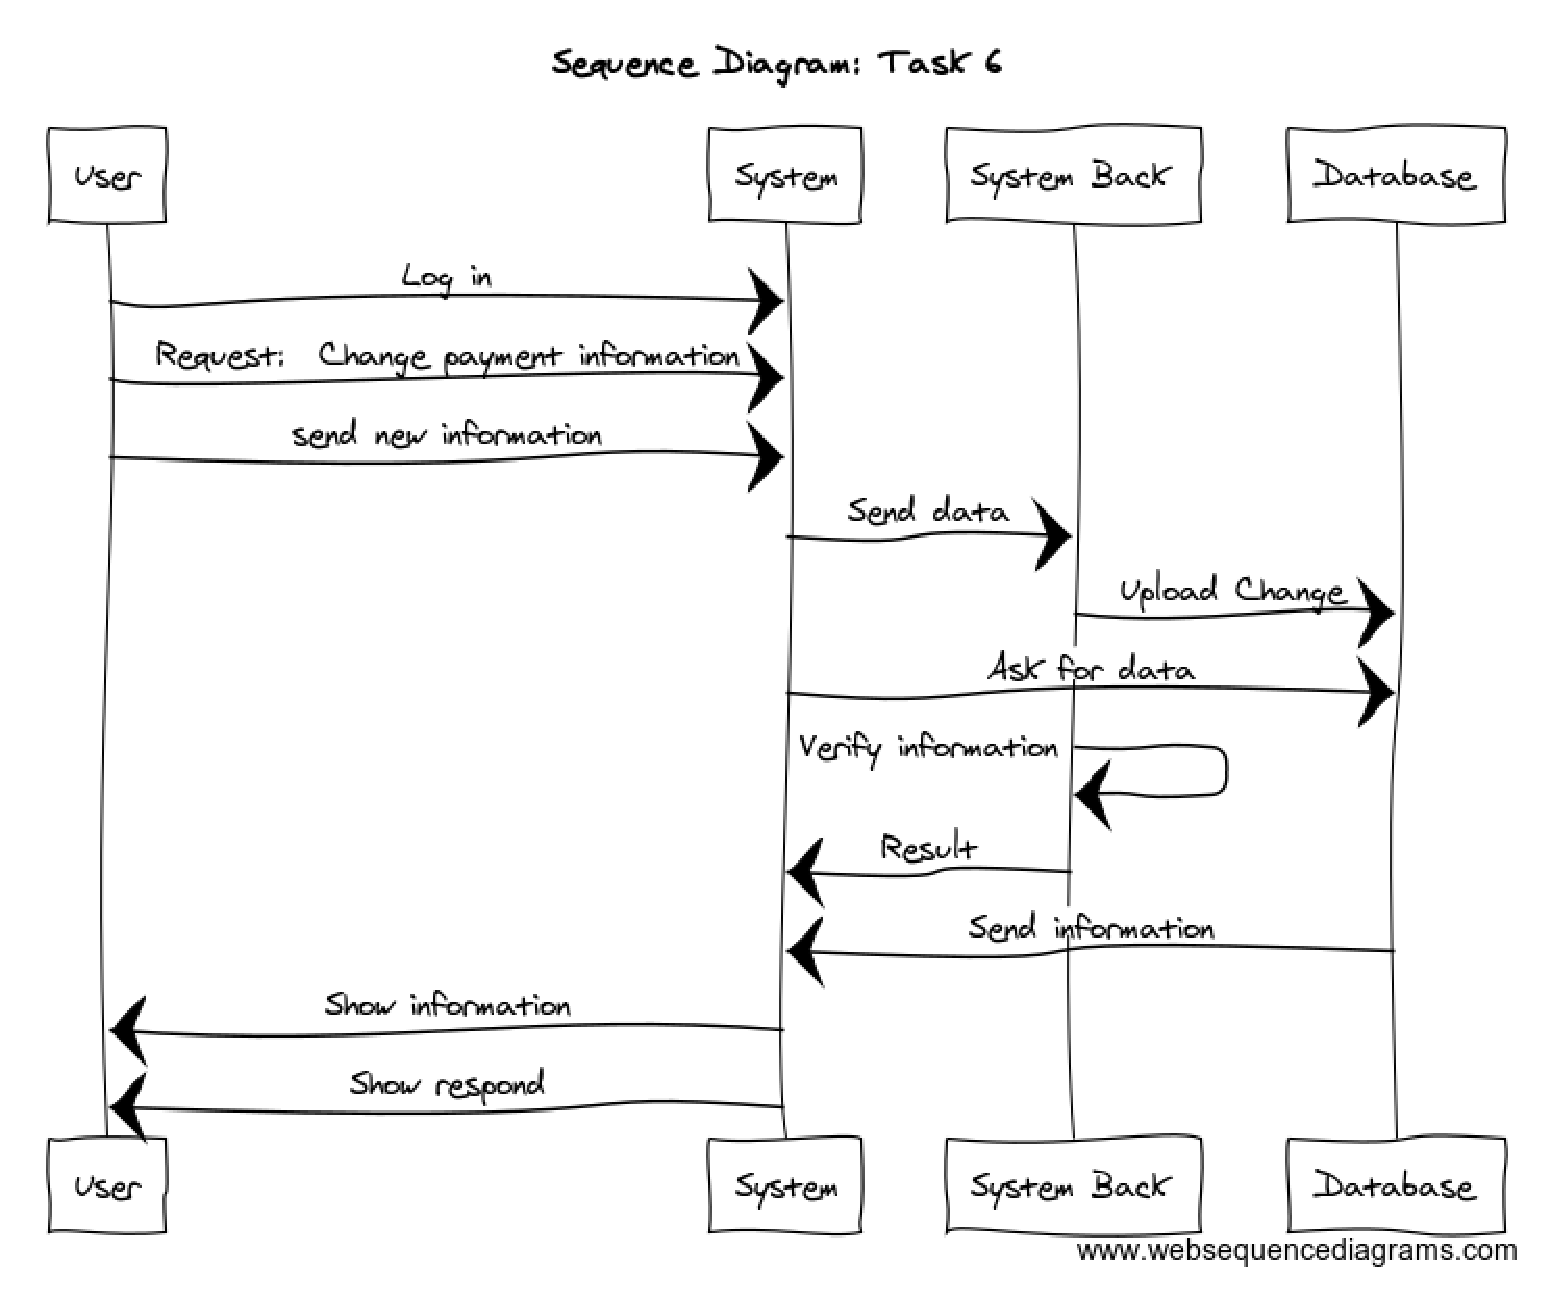
\includegraphics[width=16cm]{story6.eps}
		\clearpage
 		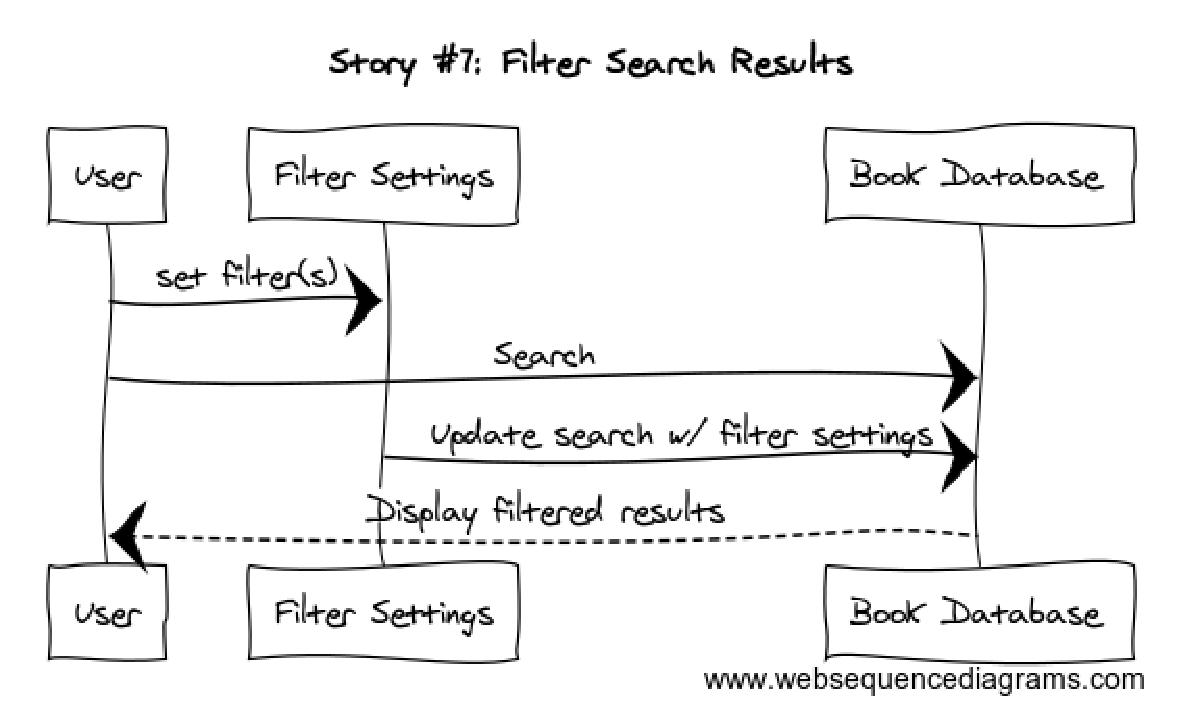
\includegraphics[width=16cm]{story7.eps}
 		\clearpage
 		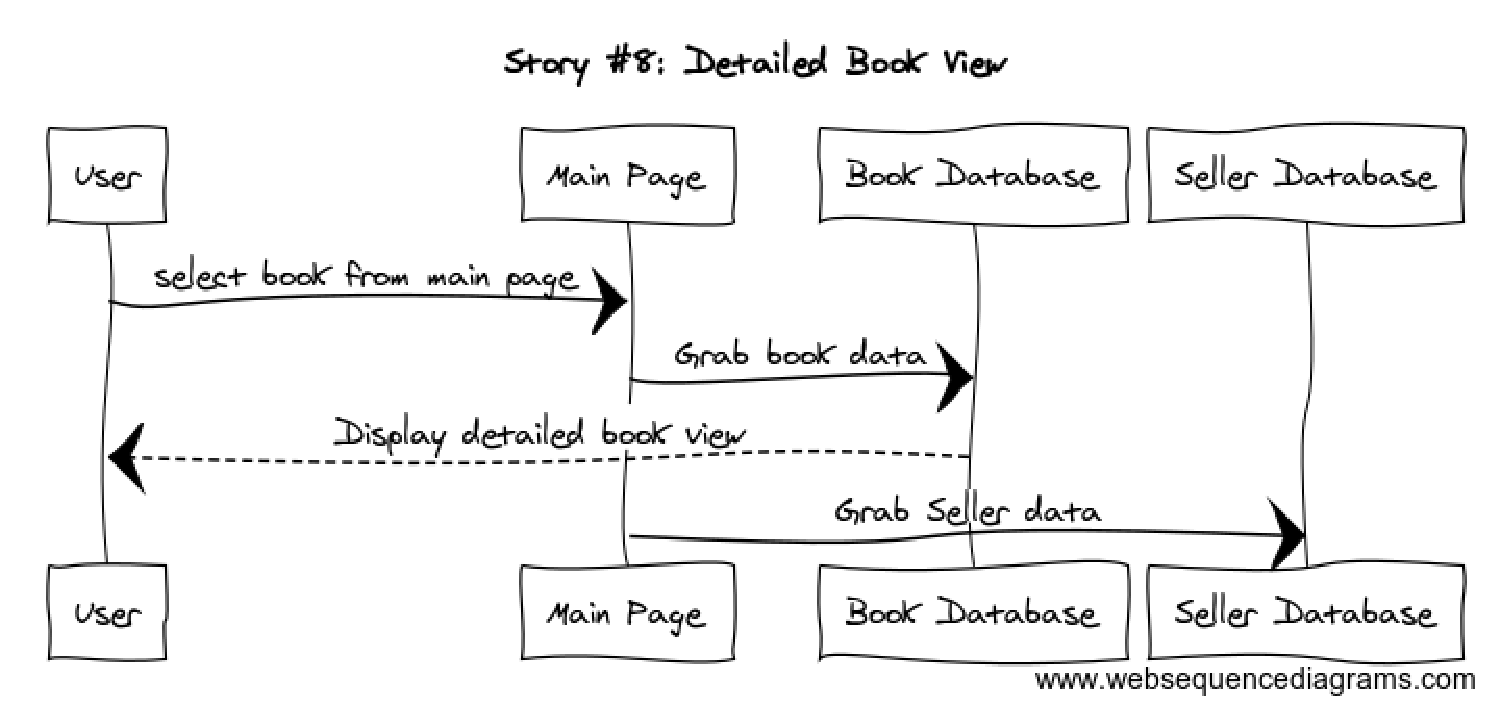
\includegraphics[width=16cm]{story8.eps}
 		\clearpage
 		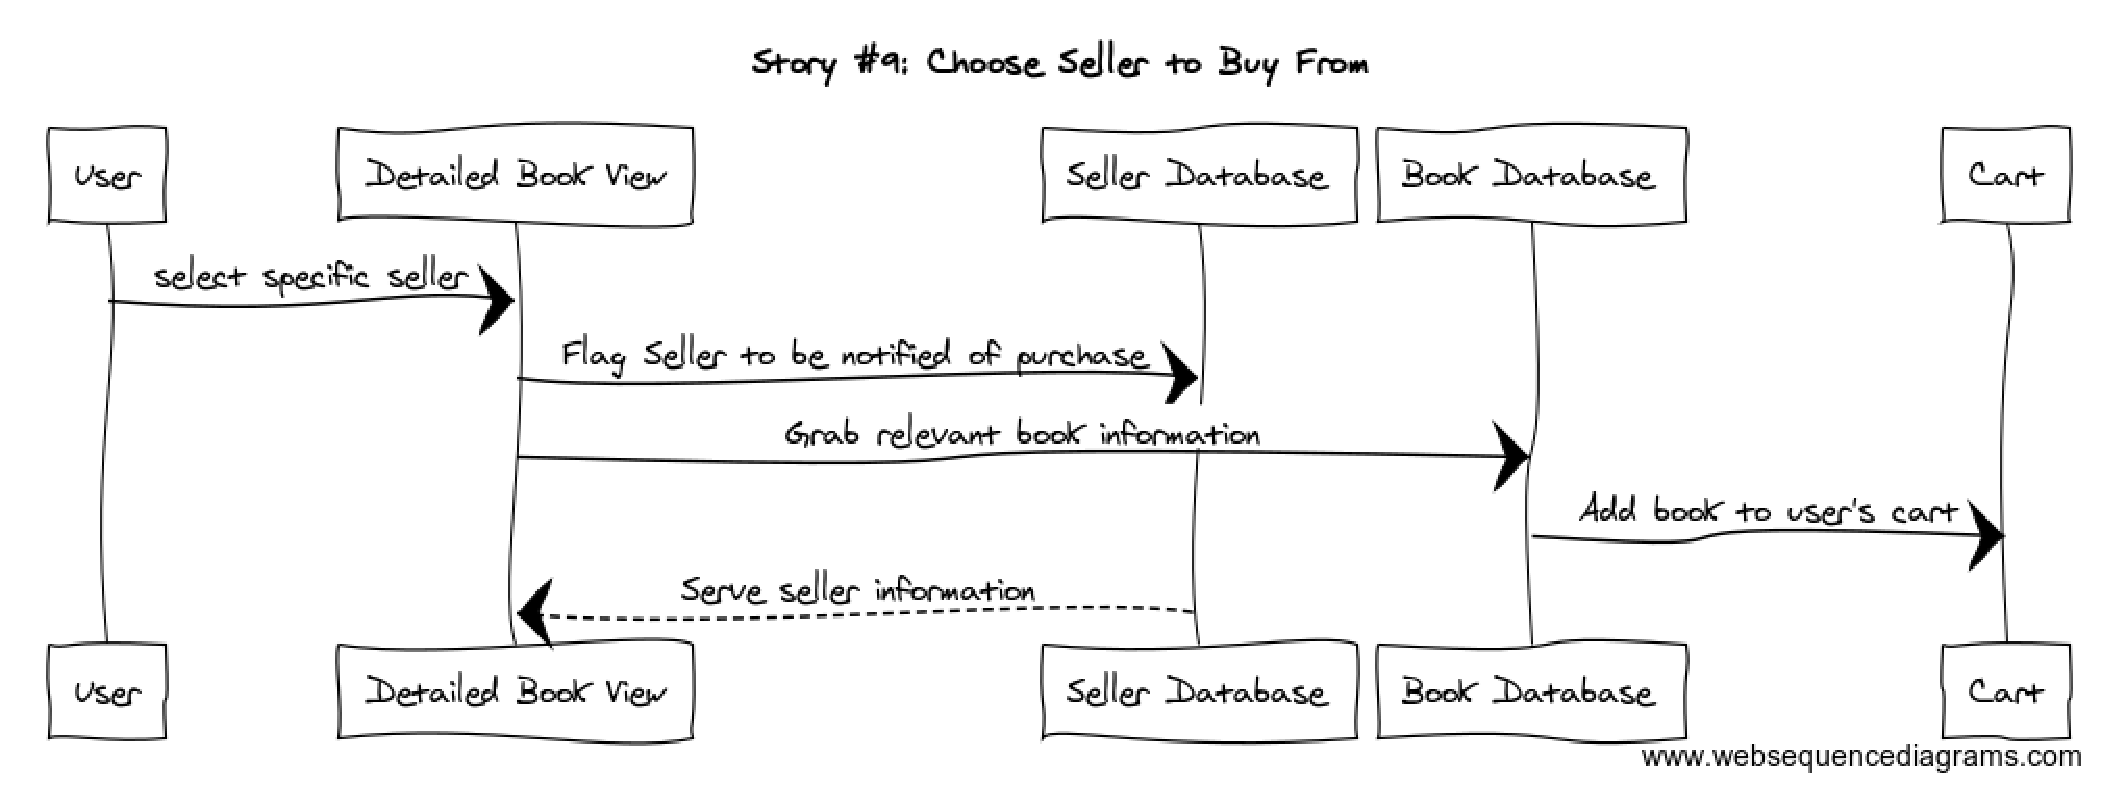
\includegraphics[width=17cm]{story9.eps}
 		%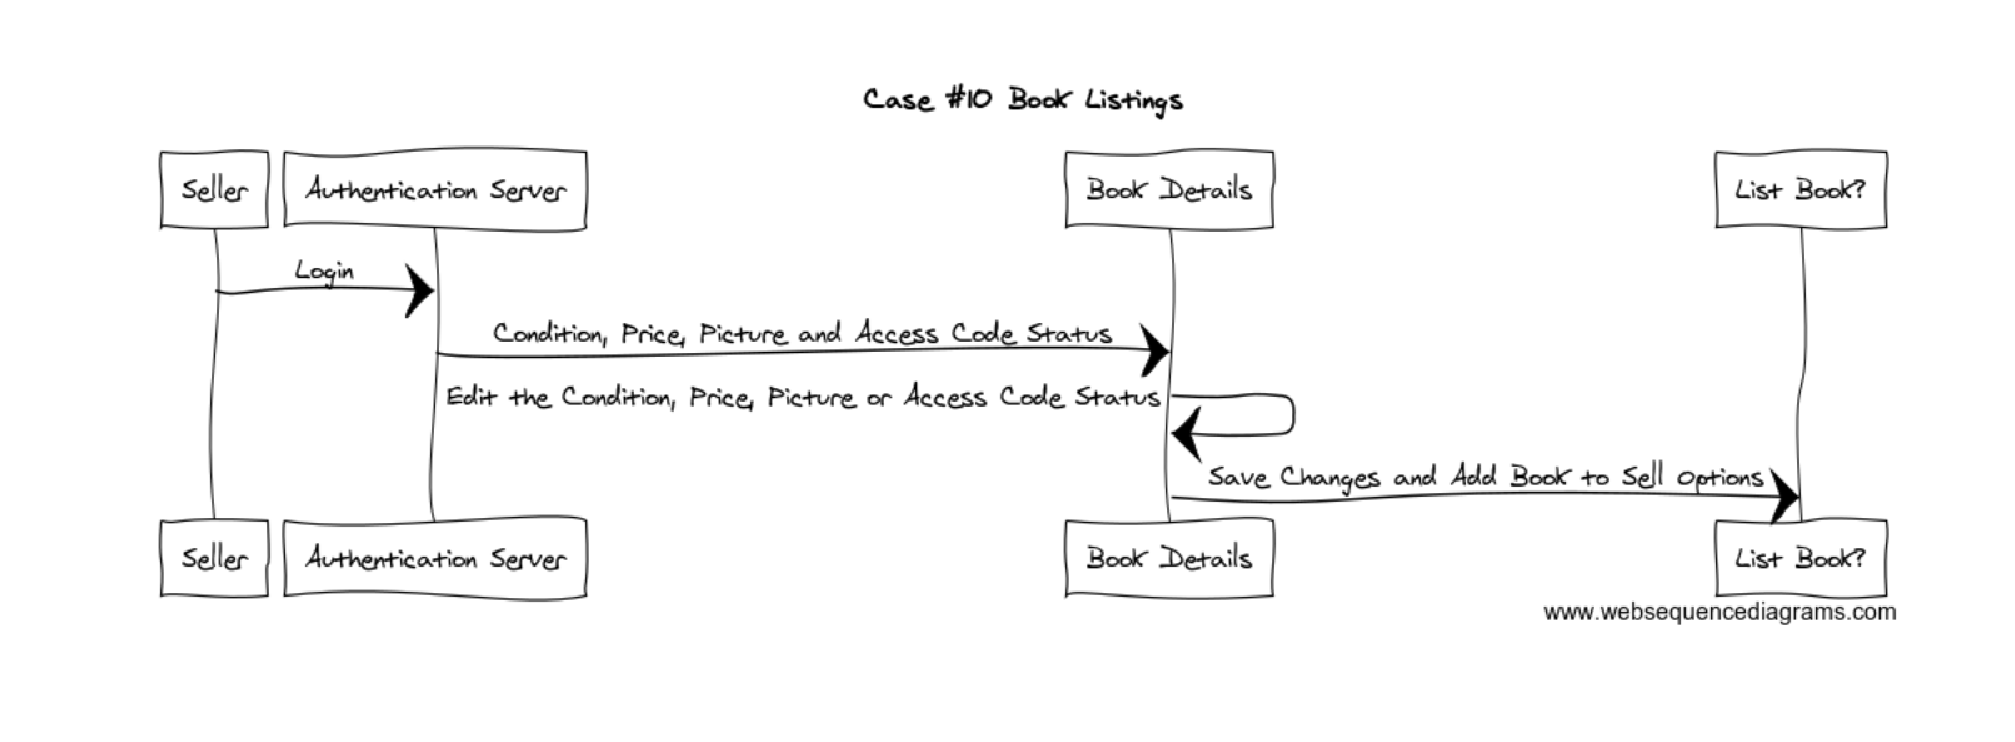
\includegraphics[width=16cm]{story10.eps}
 		%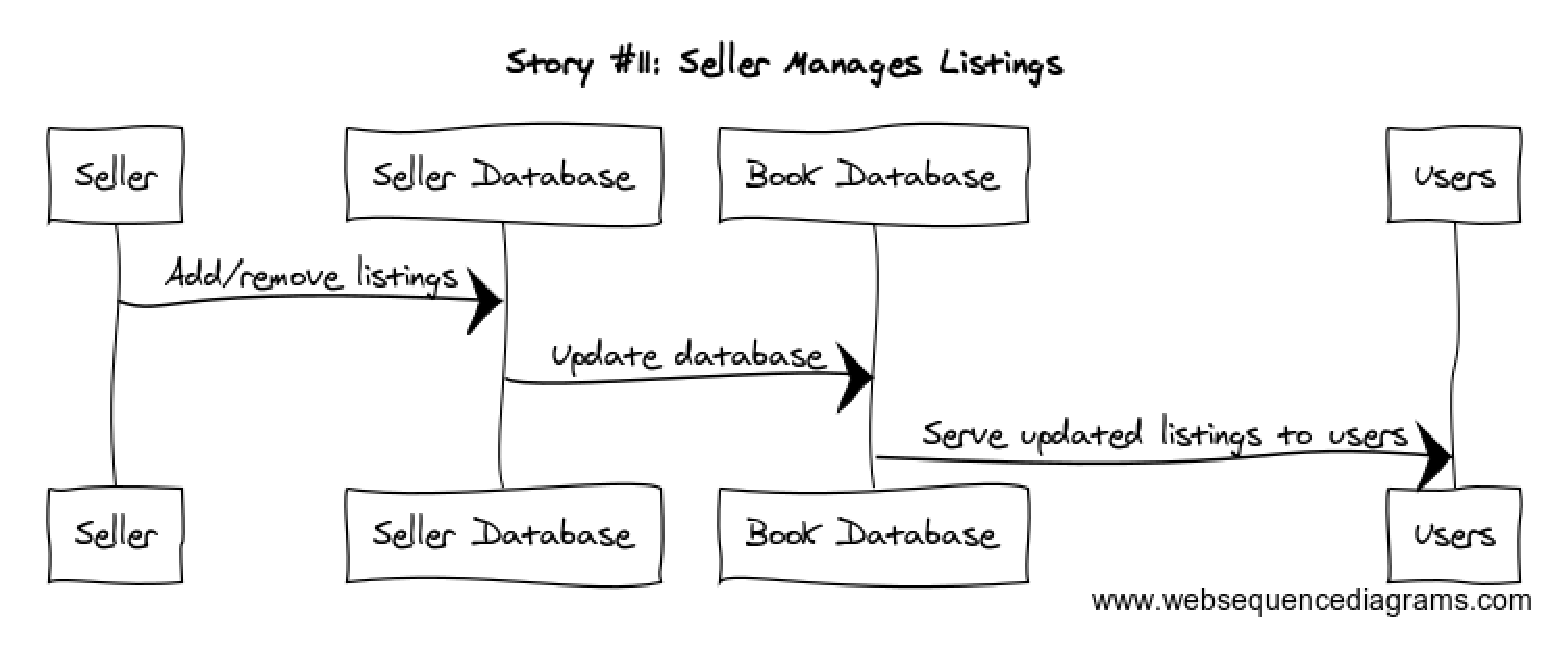
\includegraphics[width=16cm]{story11.eps}



	\section{The Stories due Next Week}
		\begin{itemize}
		\item Story 2: As a User I can add textbooks to the cart so that I can keep track of the books I am interested in.

		\item Story 3: As a User I can remove textbooks I no longer want from the cart.

		\item Story 8: As a User I can select a specific book so that I can view detailed information on it.
		\end{itemize}
		We decided to work on these particular user stories next week because they represent a baseline implementation of our project. 
		Our search and seller user stories are dependent on the existence of a book database and schema for the user to buy books. 
		We will write basic HTML for the main page and get some sample books encoded into our database.
		\subsection{Organization}
		HTML Framework: Cody and Cong \par
		Book Database: Andrew and Jacob \par
		Cart Interface/Record: Mingyu \par

		We should be able to work on the HTML and book database simultaneously. 
		After we have a working implementation of those, then we can get a simple cart interface integrated with them.



	\section{Meeting Report}
		\subsection{Progress Made}
		This week we were able to have everyone come together for our weekly meeting. 
		Together we discussed how we should best divide up the project as well as came up with several user stories that we could utilize. 
		As we worked separately on our tasks, we were sure to keep everyone informed about what we were doing and what our next steps were through our group text. 
		We have continued to use google drive for organizing the differents parts of the project.  

		\subsection{Plans/Goals for Next Week}
		We assume that next weeks project will build further off of this one, but as of yet we have received no information about it. 
		We should have it by friday in which we will get together and discuss what is needed.

		\subsection{Contributions of Each Member}
		\quad User Stories--All Members \par
		UML Sequence Diagrams/Spikes--All Members \par
		Corresponding Tasks--Cong \par
		The Stories due Next Week--Jacob \par
		Meeting Report--Andrew \par
		LaTeX--Jacob

		\subsection{Customer}
		The customer was very helpful with coming up with the user stories that we would use for this project. 
		They agreed with the ones that we were able to come up with as well as helped come up with others.

	\end {document}
	
